
\begin{opin}{\guscolor}{Gustavo}


\subsubsection{¿Qué es innovar en educación para ti?}
Innovar en educación para mí sería buscar cómo cambiar la forma tradicional de impartir las asignaturas para intentar que los alumnos se sientan más atraídos y puedan retener lo aprendido si no es para el resto de su vidas, al menos durante el mayor tiempo posible y así evitar lo que ocurre en muchos casos de que los alumnos aprueban los exámenes y se olvidan.


\subsubsection{Expectativas iniciales de la asignatura}
Personalmente considero que me encuentro entre ese perfil de alumno que aprueba un examen y se olvida casi por completo de  lo estudiado. Es cierto que esta situación se acentuaba cuando las asignaturas de las que me examinaban eran de memorizar. Con las matemáticas era algo diferente porque era necesario conocer la base para seguir avanzando en los cursos posteriores, los cuales además servían de recordatorio de lo estudiado.


Dicho esto, cuando leí el título de esta asignatura (\textit{Innovación Educativa y TICs aplicadas a la enseñanza de las Matemáticas}) me dio la sensación de que me iba a conocer cuáles son las nuevas metodologías de trabajo innovadoras que se están poniendo de moda y que son tan eficaces para el aprendizaje como las metodologías tradicionales. Estas nuevas metodologías docentes incluirían cambios drásticos con respecto a la metodología tradicional. También me imaginaba que se haría mucho hincapié en el uso de las nuevas tecnologías dado que facilita la labor para el docente y es una herramienta muy práctica en el aprendizaje.


Sobre el uso de las TICs en general me gustaría añadir una opinión personal. Tengo la sensación de que hay una tendencia generalizada de pensamiento que opina que con las TICs se va a poder hacer todo. Considero que hay que tener mucho cuidado con el uso de las tecnologías para todo. Las TICs sólo sirven cuando ayudan a realizar una determinada labor. Por poner un ejemplo simple, hay ocasiones en las que las TICs son tan complicadas de usar que no solo no ayudan sino que perjudican.

\end{opin}

\begin{opin}{\victorcolor}{Víctor}

\subsubsection{¿Qué es innovar en educación?}

Hacer las cosas de otra manera. "Si siempre haces lo mismo, no esperes resultados distintos." decía Einstein y para mi innovar es hacer de manera distinta teniendo como objetivo resultados distintos.


Tras comentar en clase la idea de innovación, he descubierto que hay otro aspecto muy importante: que sea un cambio duradero con mucha adopción.
%
Si es un cambio que no mejora las cosas, no es una innovación. 
%
Si nadie está dispuesto a adoptar la nueva forma, tampoco es una innovación.

En esta clase escuché por primera vez el término \index{Educación bulímica}\textbf{educación bulímica}, que significa \textit{Estudio para vomitar en el examen}.


\subsubsection{Expectativas de la asignatura}


Mis expectativas para la asignatura son muy altas, ya que la innovación es fundamental de cara a la profesión docente.
%
Para desarrollarme como buen docente necesito principalmente 2 cosas:
\begin{itemize}
	\item Ser capaz de innovar.
 	\item Estar atento de las innovaciones de otras personas.
 \end{itemize} 

Espero que esta asignatura me ayude a pontenciar mi capacidad innovadora y a conocer recursos con los que innovar en clase, aprovechando las buenas ideas de otras personas.


Estudiando un informe sobre la visión que se tiene de las matemáticas veo resultados que me resultan sorprendentes. 
%
Quien rechaza las mates se hace, no nace. En primaria nadie rechaza las mates, en Secundaria sí.
%
Además, todas las personas reconocen que las matemáticas son realmente útiles, quienes se les dan bien cómo quienes no se les dan bien.
%
A quien le gustan las mates, las consideran fáciles. A quién no le gustan, las consideran difíciles. 50\% de alumnos que rechazan las mates es por culpa de los malos profesores. 30\% de alumnos que no rechazan las mates es gracias a sus profesores. 

Estos datos (y los demás que estuvimos comentando en clase) me hacen darme cuenta de lo fundamental de mi labor y me han hecho tomar conciencia de la responsabilidad que lleva esta profesión. Al fin y al cabo, como dice Ben Parker \textit{un gran poder conlleva una gran responsabilidad}.


\end{opin}

\begin{opin}{\pedrocolor}{Pedro}

\subsubsection{Expectativas iniciales de la asignatura}

En la primera semana del Máster ya fui consciente de mis carencias oratorias, dado mi perfil eminentemente técnico. Por lo tanto, esta asignatura se presenta como un “Recurso” que puede potenciar mis habilidades como educador, por su proximidad al campo científico del que procedo.

Dado que actualmente nos movemos en “la era 3.0”, veo necesario el empleo de nuevas técnicas para llegar mejor al alumnado, permitiendo un mejor desarrollo cognitivo que les permita razonar de forma lógica ante su entorno. 

Mi principal objetivo, al finalizar la asignatura, es conseguir adquirir las nociones necesarias para lograr el empleo de nuevas técnicas educativas y aplicarlas en un futuro a mis alumnos, intentando conseguir con ello una mejor compresión de los conceptos matemáticos.

\subsubsection{¿Qué es innovar en educación?}

Cuando hablamos de “Innovación educativa”, estamos introduciendo cambios en los patrones tradicionales de la educación, que conlleva una mejora del mismo. Para llevarlo a cabo, debemos pasar por un proceso de selección, organización y utilización creativa de los recursos humanos y materiales, que den como resultado los objetivos marcados. (Richland, citado por Moreno, 1995).

Tras la lectura de todas las definiciones de Innovación educativa que han dado alumnos de otros años, me gustaría aportar mi propia definición.

“La innovación educativa nace como resultado de un proceso que consiste en la observación y estudio de manera objetiva de las situaciones que se dan en el aula. Teniendo como resultado final la búsqueda de la mejora del proceso de aprendizaje del alumnado, mediante materiales y técnicas nuevas.

Considero que la mejor manera para demostrar que nuestro intento de Innovación Educativa en el aula tiene efectos positivos en el aprendizaje, es lograr captar la atención del alumno.

Con la llegada de la LOGSE, se comienza a pedir a los profesores de secundaria un conocimiento  didáctico sobre la materia que van a impartir. Sus críticas principales radican en el corto período de formación y la consideración de dicho proceso como un mero trámite.

La LOE habla por primera vez sobre la importancia de enseñar competencias y no contenidos, entendiendo por competencias básicas aquellas habilidades que todos los alumnos deben haber alcanzado al finalizar la Educación Secundaria Obligatoria. Como aspecto negativo, esta ley contempla la posibilidad de pasar de curso con materias suspensas, lo que supone potenciar el error de construir conocimientos justo encima de lagunas arrastradas de cursos anteriores.

Con la implantación del Plan Bolonia, se logra dar al Profesorado de Secundaria la necesaria formación teórica (académica y pedagógica) y práctica.  No obstante, es fundamental que el profesor de matemáticas:

\begin{itemize}
%\vspace{-0.2cm}
\item Se encuentre inmerso en un proceso continuo de actualización (científica y didáctica), lográndose mediante la investigación educativa y acercamiento a nuevas TICs. 
%\vspace{-0.2cm}
\item Se encuentre motivado por la asignatura. 
%\vspace{-0.2cm}
\item Conozca los diferentes enfoques que se puede dar a la asignatura, sin limitarse a formalismos. 
%\vspace{-0.2cm}
\item Elija el metodo adecuado de enseñanza para cada etapa o situación de aprendizaje. 

\end{itemize}

Me llama especialmente la atención los resultados arrojados por los estudios de evaluación educativa (PISA o TIMSS), mostrando un deterioro significativo de la enseñanza matemática pese a las reformas educativas que se han llevado a cabo. Y me pregunto: ¿Qué podemos hacer el profesorado para cambiar esta situación? ¿La utilización de recursos educativos en el aula mejoraría el proceso de enseñanza-aprendizaje? ¿Hace falta ser un experto para el uso básico de TICs?


\begin{minipage}[hbtp]{1.0\linewidth}
\centering
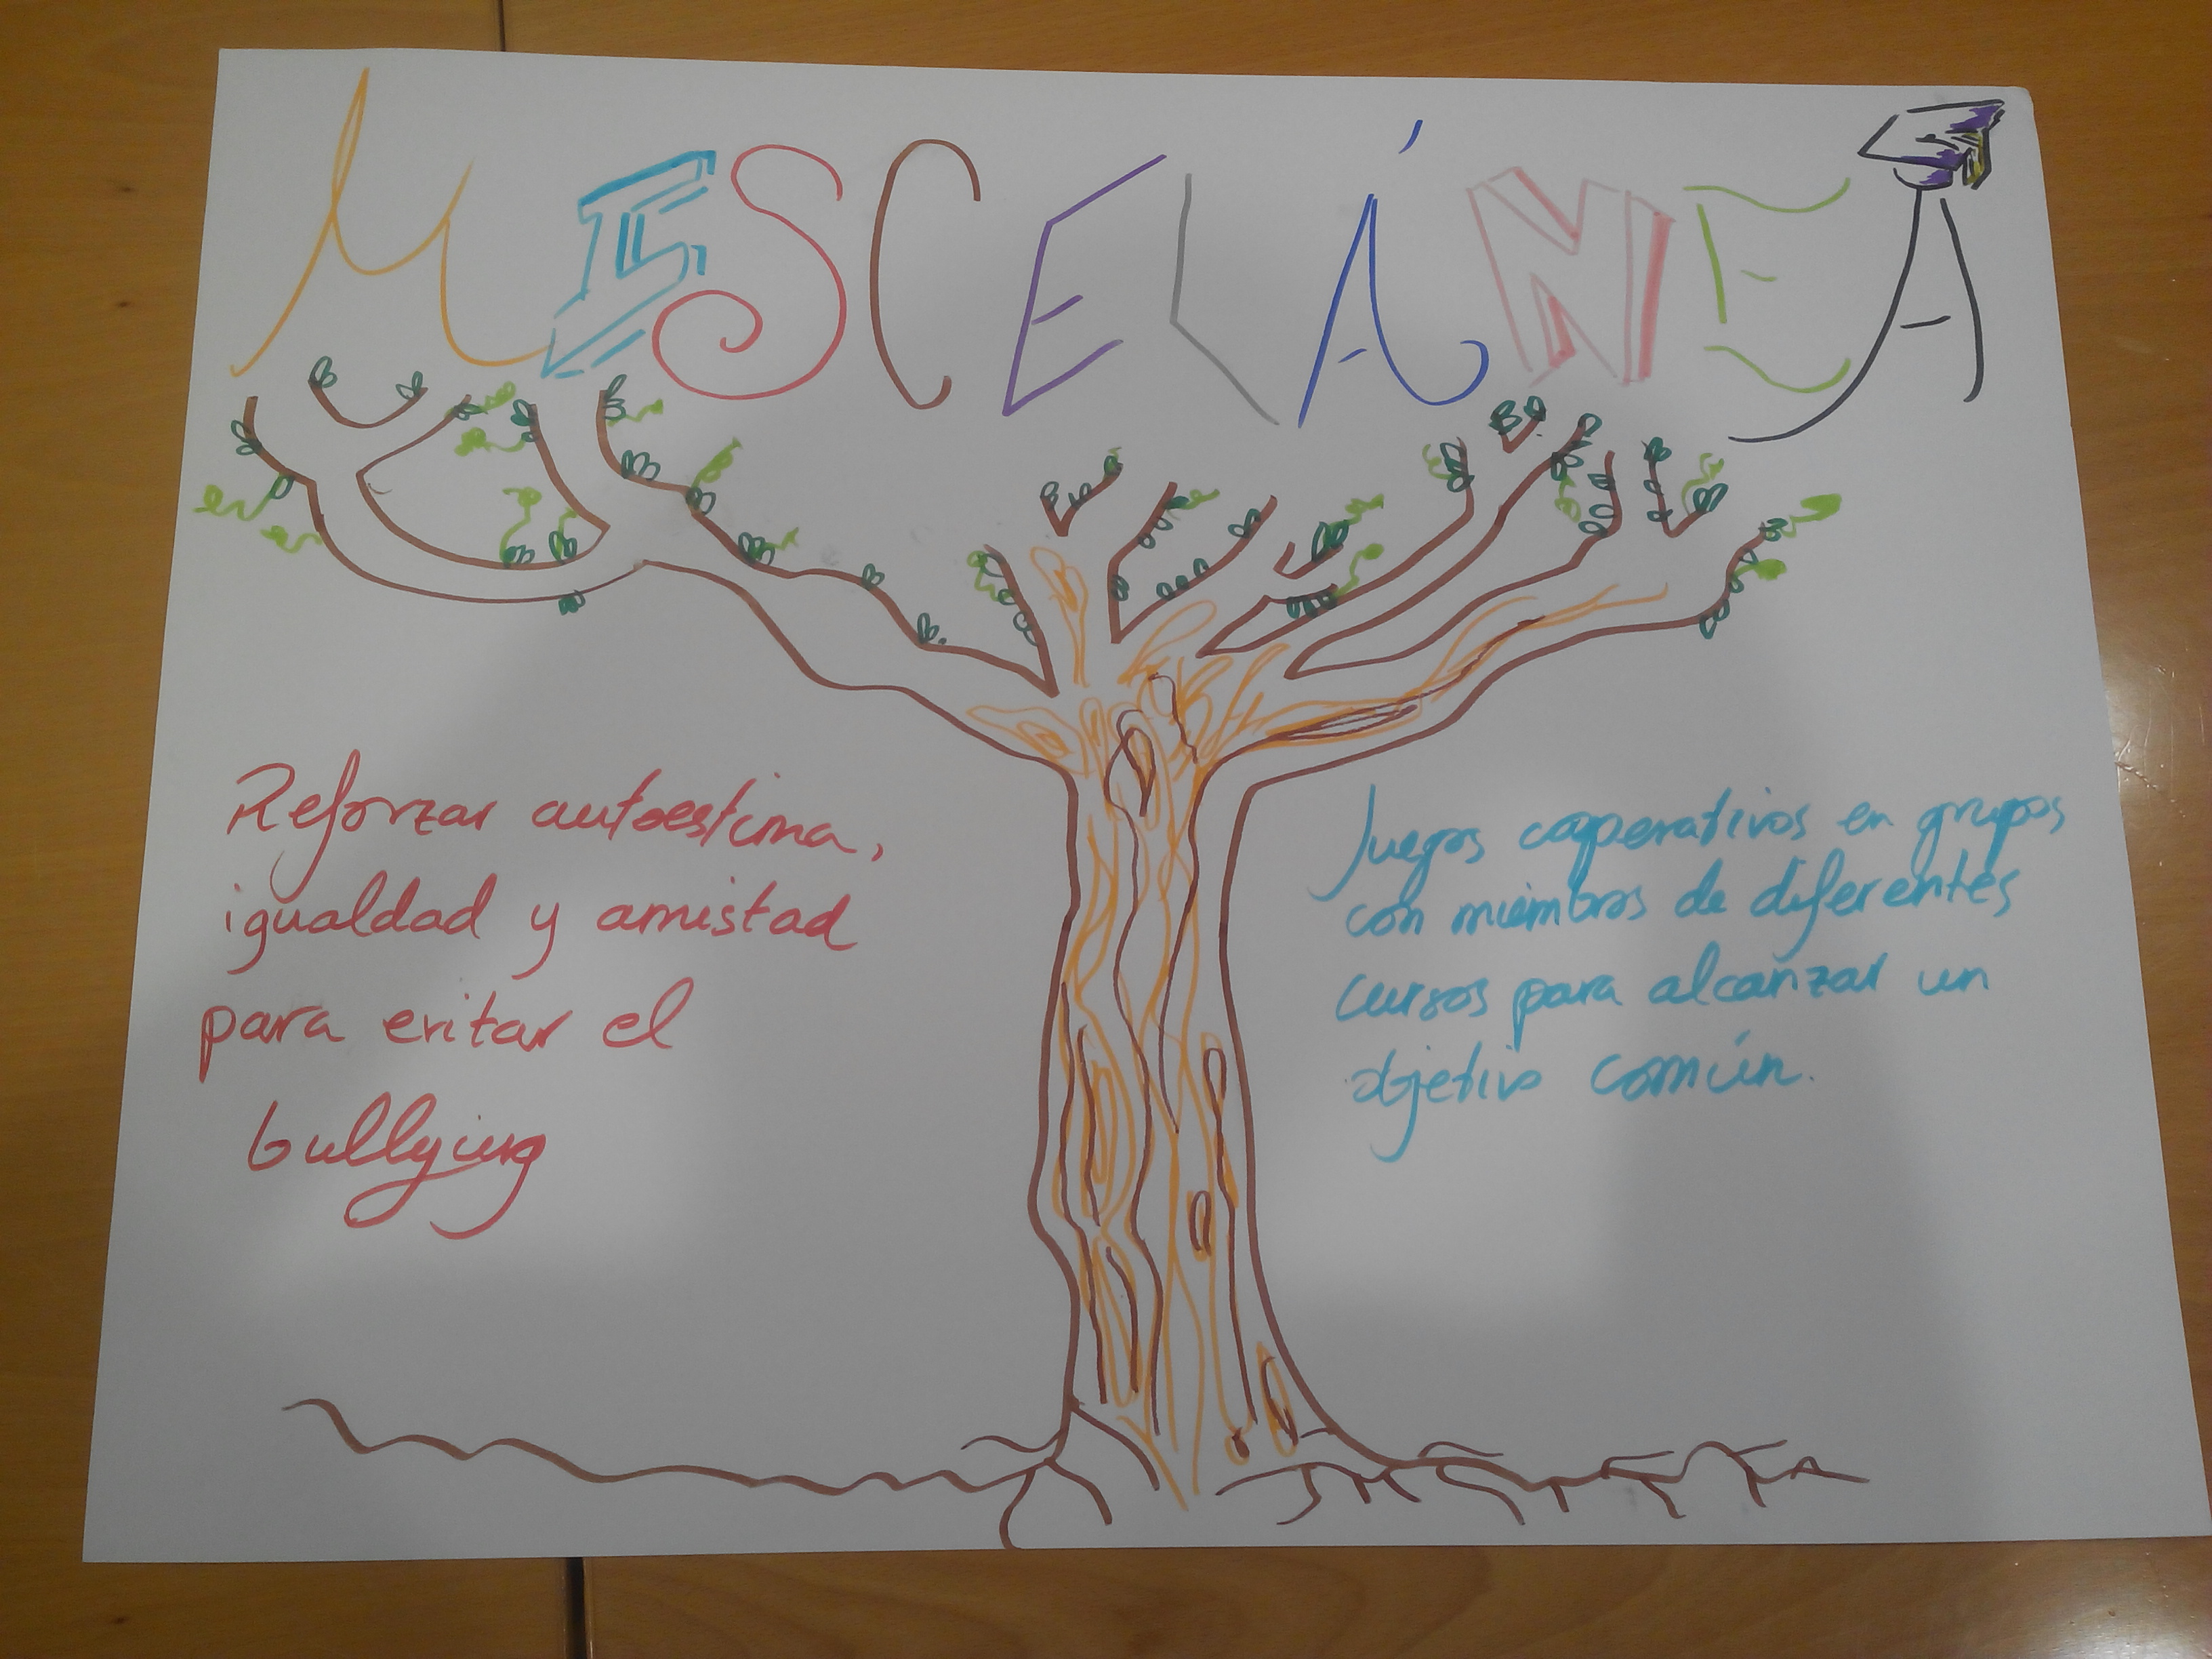
\includegraphics[scale=0.1]{img/pedro1.jpg}
\captionof{figure}{Actividad Jornada Metodologías Activas de educación en el aula con Irene Ros \\ ¿Qué haríais para mejorar la educación?}
\end{minipage}

\end{opin}

\begin{opin}{\virgicolor}{Virginia}
.


\end{opin}
